\documentclass[11pt,letterpaper]{article}
\usepackage[utf8]{inputenc}
\usepackage[T1]{fontenc}
\usepackage{mathptmx}
\usepackage[letterpaper,left=1.25in,right=1.25in,top=1.2in,bottom=1.2in,headheight=14pt]{geometry}
\usepackage{microtype}
\usepackage{amsmath,amssymb,amsthm,mathtools,bm}
\usepackage{graphicx,booktabs,array,multirow,float}
\usepackage{xcolor}
\usepackage{enumitem}
\usepackage[labelfont=bf,labelsep=colon,font=small,skip=4pt]{caption}
\usepackage{subcaption}
\usepackage{fancyhdr}
\usepackage{titlesec}
\usepackage{listings}
\usepackage{tikz}
\usetikzlibrary{arrows.meta,positioning,calc}
\usepackage[authoryear,round]{natbib}
\definecolor{linkcol}{HTML}{2B3A8F}
\usepackage[colorlinks=true,linkcolor=linkcol,citecolor=linkcol,urlcolor=linkcol]{hyperref}
\usepackage[capitalise,noabbrev]{cleveref}

\pagestyle{fancy}\fancyhf{}
\lhead{\small Technical report.}
\cfoot{\small\thepage}
\renewcommand{\headrulewidth}{0.5pt}
\setlength{\parskip}{4pt plus 1pt}\setlength{\parindent}{0pt}
\titleformat{\section}{\large\bfseries}{\thesection}{0.8em}{}
\titleformat{\subsection}{\normalsize\bfseries}{\thesubsection}{0.8em}{}
\titleformat{\subsubsection}{\normalsize\bfseries\itshape}{\thesubsubsection}{0.8em}{}
\titlespacing*{\section}{0pt}{16pt}{6pt}\titlespacing*{\subsection}{0pt}{12pt}{4pt}
\setlist{itemsep=1pt,topsep=3pt}
\setlength{\emergencystretch}{2em}

\theoremstyle{definition}
\newtheorem{definition}{Definition}
\theoremstyle{remark}
\newtheorem{remark}{Remark}

\lstset{basicstyle=\ttfamily\small,breaklines=true,frame=single,framerule=0.3pt,
  xleftmargin=4pt,xrightmargin=4pt,columns=fullflexible,keepspaces=true,showstringspaces=false}

% title block: \reporttitle{title}{subtitle}{authors}{affiliation line}
\newcommand{\reporttitle}[4]{%
\begin{center}
{\LARGE\bfseries #1\\[4pt]
\Large #2\par}
\vspace{1.4em}
{\bfseries\color{linkcol}\large #3}\\[0.4em]
{\small #4}\par
\vspace{1.2em}
\end{center}}
\newcommand{\abstractblock}[1]{%
\begin{center}\textbf{Abstract}\end{center}
\vspace{-0.4em}
\begin{quote}\small #1\end{quote}
\vspace{0.4em}}

\begin{document}
\reporttitle{Matamata: A Hexagonal-Scute Wheel for Planetary Rovers}{Design and a 25\% Scale Manufacturing Prototype}{Juan Fernando Casta\~no}{NYU Abu Dhabi \quad ENGR-UH 2113, Spring 2025}

\abstractblock{The aluminium wheels of Mars rovers have been damaged at the corners of their wave-shaped treads. We propose a tread made of hexagonal scutes, after the shell of the matamata turtle (\emph{Chelus fimbriata}), with 4\,cm sides at full scale, so that load is carried by flat faces and not by corners. The core keeps the Perseverance architecture with added ribs, and the curved connector bars become thicker straight bars. We built a 25\% scale prototype to find out whether the design can be made with tools available to a student: a 3D-printed tread, a laser-cut stacked core and a connector frame cut in one piece. Three print iterations showed that 90$^\circ$ overhangs fail on a desktop printer and that a 45$^\circ$ chamfer on the tread and the inner rim fixes it. Stacking laser-cut layers avoided printing the core, and joining the six bars into one frame kept them from breaking during cutting. The prototype cost \$64.50. We did no mechanical testing, so the design is unproven as a wheel. The full-scale materials (7075-T6 aluminium with a Nitinol coating, Ti-6Al-4V bars, 316 stainless pins) are a proposal.}

\section{Introduction}
Rover wheels are both the vehicle's suspension and its contact with the ground. On Mars the terrain is rocky enough to puncture, tear and crack thin aluminium treads; the Curiosity wheels accumulated tears and cracks over the first years of the mission \citep{arvidson2017}, and the Perseverance wheels were redesigned with a thicker skin and a shorter, more closely spaced tread pattern \citep{nasawheels}.

We ask two questions about a wheel whose tread is a field of hexagons.

\textbf{Question 1: can a hexagonal tread be arranged so that no corner carries the load alone?} The shell of the matamata turtle is covered with raised polygonal scutes. We take the idea of a surface divided into small, flat, similar elements, each of which can bear on the ground without a sharp edge being the only contact.

\textbf{Question 2: can the geometry be made at small scale with ordinary tools?} A design that cannot be manufactured cannot be tested. The prototype exists to answer this question and no other.

\textbf{What we find.} The design can be made at 25\% scale for \$64.50, but only after three print iterations (two chamfer changes) and two changes to the laser-cut parts (\cref{tab:iter}). We make no claim about strength, traction or fatigue life.

\textbf{Contributions.} We do not claim a validated wheel. The contributions are:
\begin{enumerate}
\item a wheel concept with a hexagonal-scute tread, ribbed core and straight connector bars (\cref{sec:design});
\item a record of what had to change to make it at 25\% scale, and why (\cref{sec:proto});
\item the CAD, the laser-cut and print geometry, and photographs of the prototype in one repository (\cref{sec:avail}).
\end{enumerate}

\section{Background}\label{sec:bg}
The wheels of the Mars Science Laboratory rover are machined from aluminium with a wave-like grouser pattern. Terrain interaction studies relate the pattern of punctures and tears to rock size and to the loading of individual grousers \citep{arvidson2017}. Perseverance kept the aluminium wheel and changed its geometry \citep{nasawheels}. Our core follows that architecture. Our change is to the tread: replacing continuous grousers with discrete scutes alters where the contact load goes.

\section{Design}\label{sec:design}
\begin{figure}[t]\centering
\begin{subfigure}{0.48\linewidth}\centering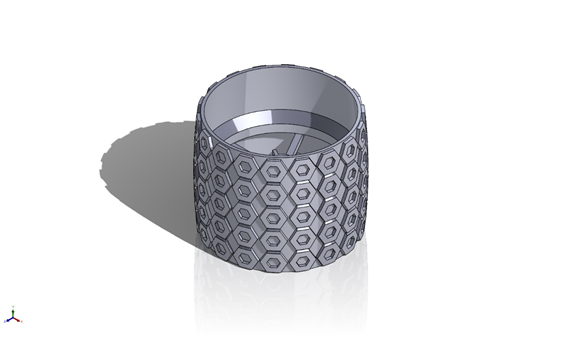
\includegraphics[width=\linewidth]{figures/cad_assembled.png}\caption{Assembled.}\end{subfigure}\hfill
\begin{subfigure}{0.48\linewidth}\centering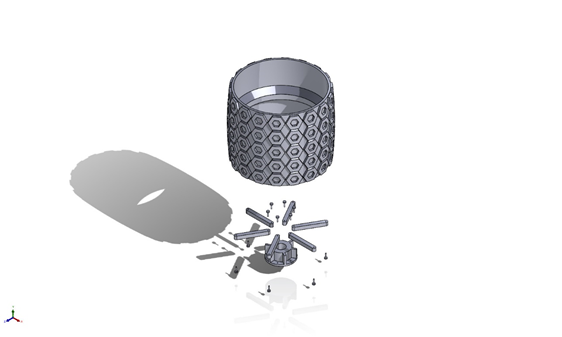
\includegraphics[width=\linewidth]{figures/cad_exploded.png}\caption{Exploded.}\end{subfigure}
\caption{CAD model of the wheel.}\label{fig:cad}
\end{figure}
\textbf{Tread.} Hexagonal scutes, 4\,cm per side at full scale, cover the rim. Each scute is a flat face, intended to bear on the ground and to spread contact stress over its area. The bevels between scutes are meant to shed regolith; we have not tested that.

\textbf{Core.} The core follows the Perseverance architecture, with ribs added.

\textbf{Connector bars.} Curved connector bars are replaced by thicker straight bars, which are simpler to cut and to check. Six of them join hub and rim.

\textbf{Full-scale materials (proposed).} 7075-T6 aluminium with a Nitinol coating for the tread, Nitinol-reinforced aluminium for the core, Ti-6Al-4V for the bars and 316 stainless steel for the pins. We selected these on the basis of published properties and did not test them.

\section{Prototype and Manufacturing}\label{sec:proto}
The prototype is built at 25\% scale from three kinds of part: a 3D-printed tread, a laser-cut core made of stacked layers, and a connector frame (\cref{fig:proto}). The bar frame measures about 450\,mm across and 50\,mm in thickness in the CAD export, and the laser-cut core layer is 135\,mm by 150\,mm.
\begin{figure}[t]\centering
\begin{subfigure}{0.32\linewidth}\centering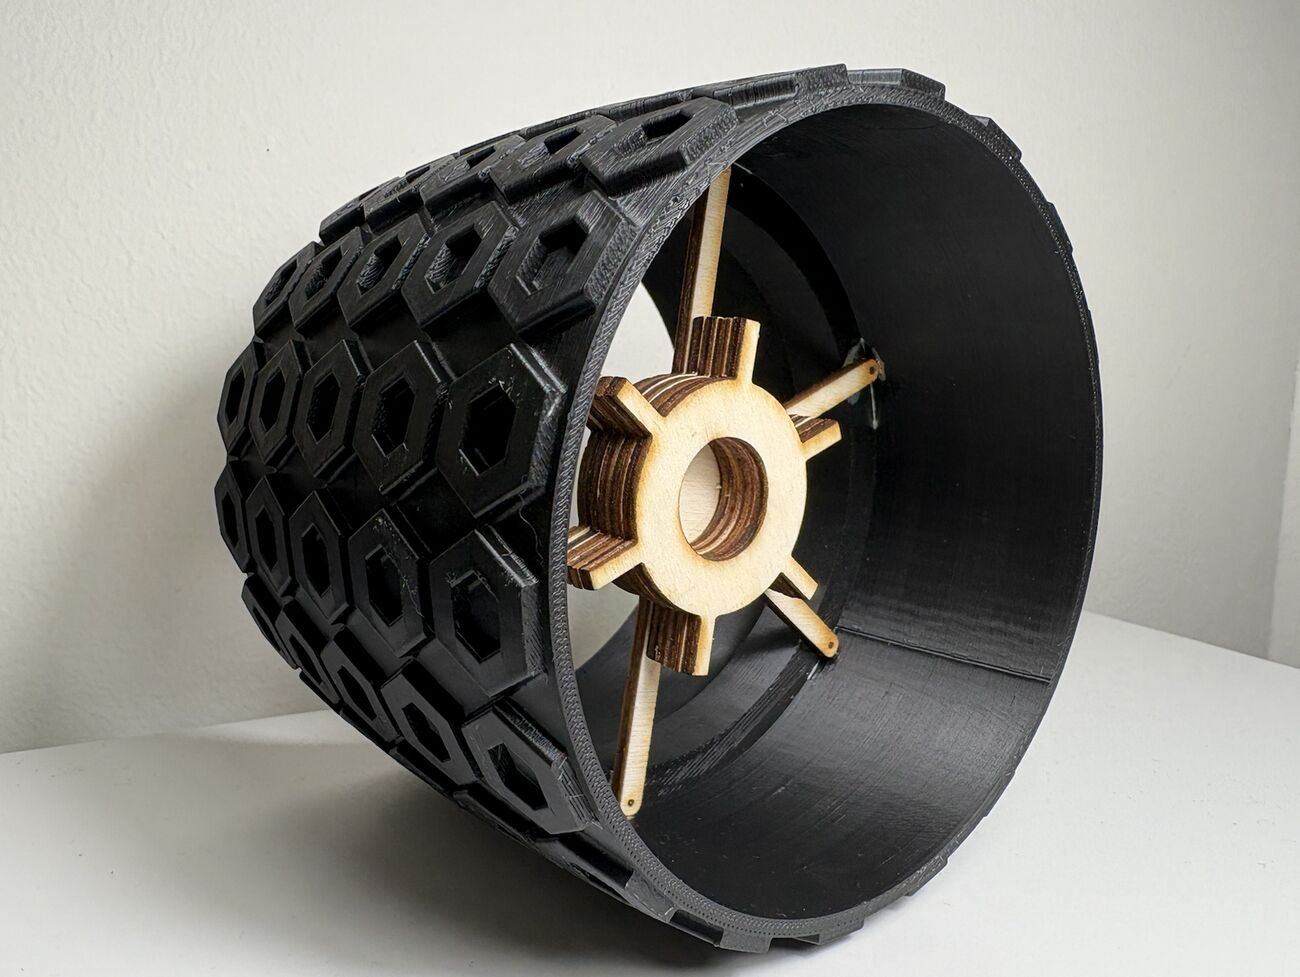
\includegraphics[width=\linewidth]{figures/proto_front.jpg}\caption{Front.}\end{subfigure}\hfill
\begin{subfigure}{0.32\linewidth}\centering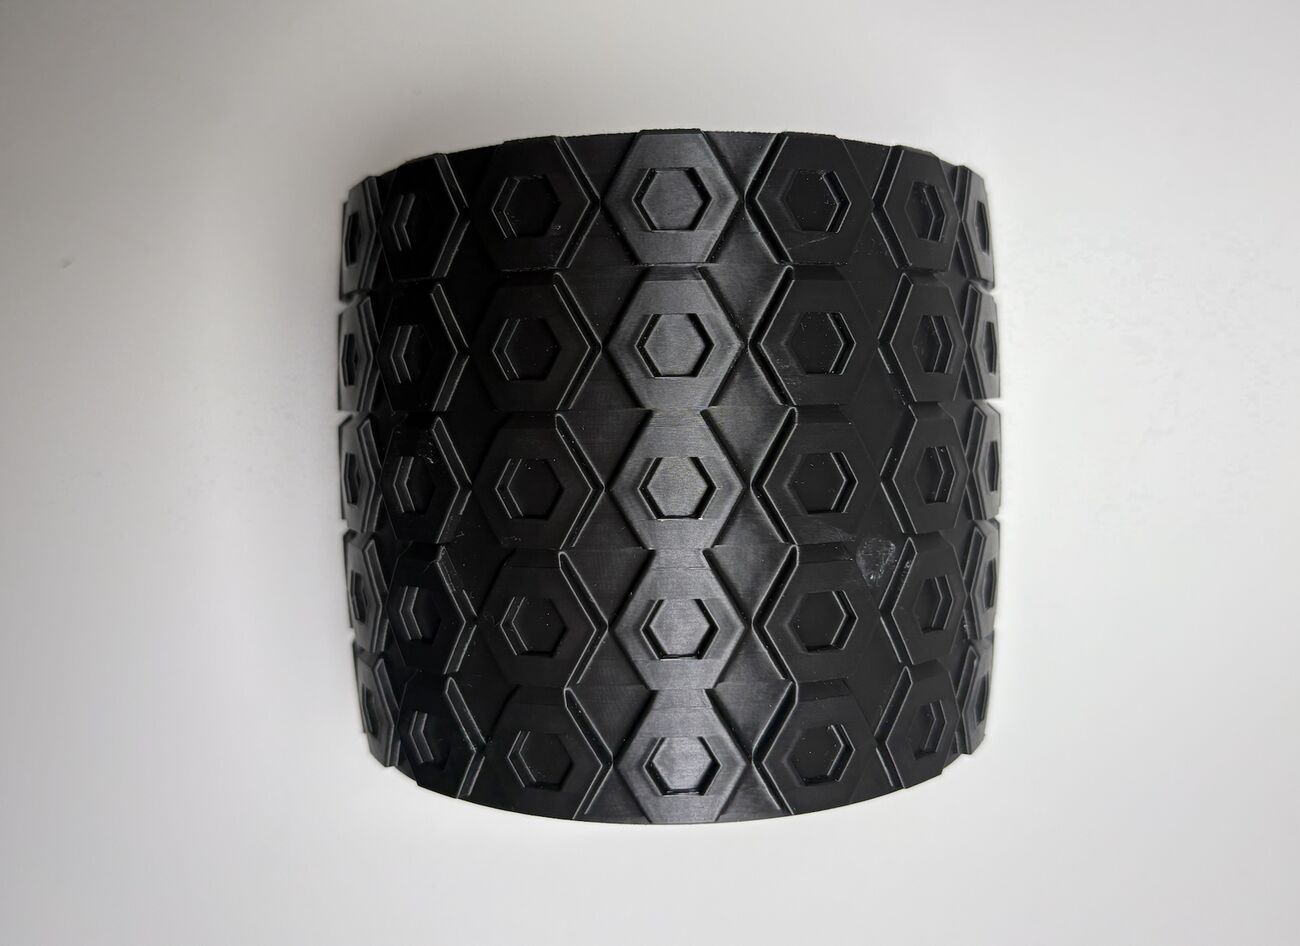
\includegraphics[width=\linewidth]{figures/proto_tread_angle.jpg}\caption{Tread.}\end{subfigure}\hfill
\begin{subfigure}{0.32\linewidth}\centering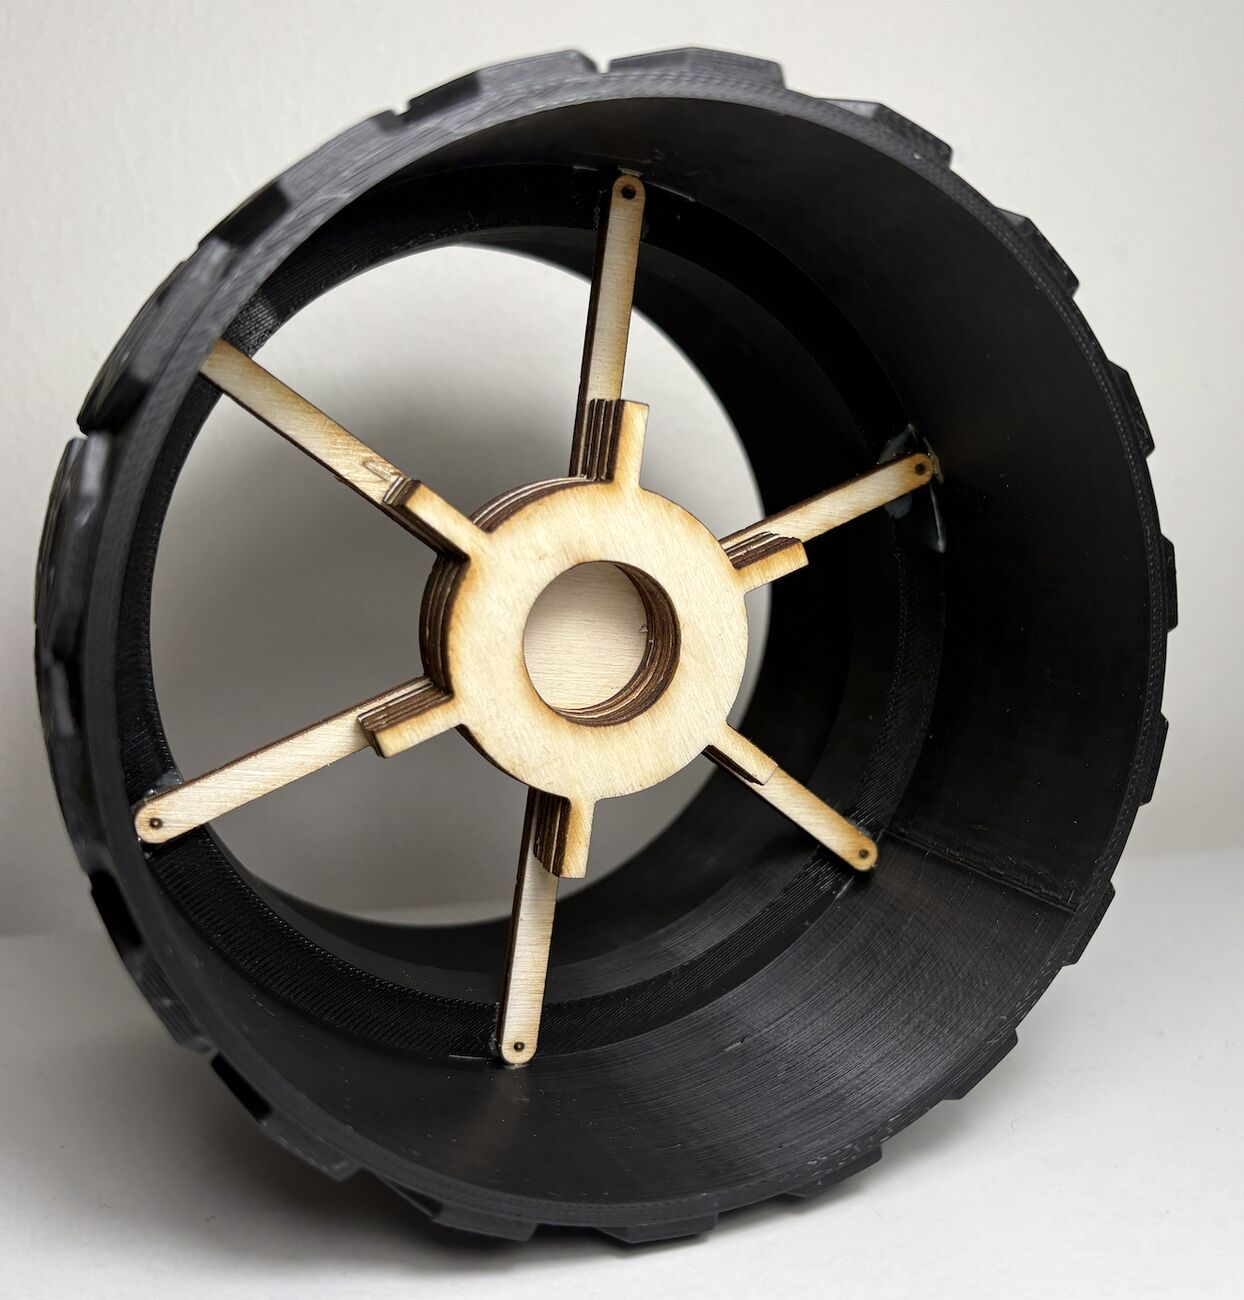
\includegraphics[width=\linewidth]{figures/proto_core.jpg}\caption{Core.}\end{subfigure}
\caption{The 25\% scale prototype.}\label{fig:proto}
\end{figure}

\begin{table}[t]\centering\small
\caption{What had to change to make the design at 25\% scale.}\label{tab:iter}
\begin{tabular}{p{1.8cm}p{5.2cm}p{6.8cm}}
\toprule
Part & Problem & Change \\
\midrule
Tread & 90$^\circ$ hexagon edges did not print & 45$^\circ$ chamfer on the lower side of each hexagon \\
Inner rim & Second print failed on overhangs & 45$^\circ$ chamfer; third print succeeded \\
Core & One-piece core wasted material & Stacked laser-cut layers, with test cylinders to set spacing \\
Bars & Loose bars broke during laser cutting & Six bars joined in one circular frame \\
Fastening & Screws not feasible at 25\% & Glued for the prototype; screws and welds kept for full scale \\
\bottomrule
\end{tabular}
\end{table}

\textbf{Cost.} The prototype cost \$64.50, counting material, processing, labour and facility use.

\section{Discussion}\label{sec:discussion}
The prototype shows that the geometry can be produced with a desktop printer and a laser cutter if overhangs are limited to 45$^\circ$ and the cut parts are connected so they survive handling. The course report attributes a 25\% reduction in wasted material to the stacked core; we did not measure it again.

\textbf{What this study does not establish.} We did not test traction, load capacity, fatigue or behaviour in loose soil. The claims that the scutes spread stress evenly and that the bevels shed regolith are design intent. Glued PLA at 25\% scale says nothing about the proposed alloys at full scale, and the joints at full scale are untested.

\textbf{Next steps.} A finite-element comparison of one scute against a conventional grouser under the same load is the cheapest next test. After that, a rolling test of the prototype on a bed of regolith simulant.

\section*{Code and data availability}\label{sec:avail}
The SolidWorks parts and assembly, the laser-cut and print geometry, and the photographs are in the repository's \texttt{cad} and \texttt{images} folders.

\bibliographystyle{plainnat}
\bibliography{references}
\end{document}
